%%%%%%%%%%%%%%%%%%%%%%%%%%%%%%%%%%%%%%%%%
% Short Sectioned Assignment LaTeX Template Version 1.0 (5/5/12)
% This template has been downloaded from: http://www.LaTeXTemplates.com
% Original author:  Frits Wenneker (http://www.howtotex.com)
% License: CC BY-NC-SA 3.0 (http://creativecommons.org/licenses/by-nc-sa/3.0/)
%%%%%%%%%%%%%%%%%%%%%%%%%%%%%%%%%%%%%%%%%

%----------------------------------------------------------------------------------------
%	PACKAGES AND OTHER DOCUMENT CONFIGURATIONS
%----------------------------------------------------------------------------------------

\documentclass[paper=a4, fontsize=11pt]{scrartcl} % A4 paper and 11pt font size

% ---- Entrada y salida de texto -----

\usepackage[T1]{fontenc} % Use 8-bit encoding that has 256 glyphs
\usepackage[utf8]{inputenc}
%\usepackage{fourier} % Use the Adobe Utopia font for the document - comment this line to return to the LaTeX default

% ---- Idioma --------

\usepackage[spanish, es-tabla]{babel} % Selecciona el español para palabras introducidas automáticamente, p.ej. "septiembre" en la fecha y especifica que se use la palabra Tabla en vez de Cuadro

% ---- Otros paquetes ----

\usepackage{url} % ,href} %para incluir URLs e hipervínculos dentro del texto (aunque hay que instalar href)
\usepackage{amsmath,amsfonts,amsthm} % Math packages
%\usepackage{graphics,graphicx, floatrow} %para incluir imágenes y notas en las imágenes
\usepackage{graphics,graphicx, float, subfig} %para incluir imágenes y colocarlas

% Para hacer tablas comlejas
%\usepackage{multirow}
%\usepackage{threeparttable}

%\usepackage{sectsty} % Allows customizing section commands
%\allsectionsfont{\centering \normalfont\scshape} % Make all sections centered, the default font and small caps

\usepackage{fancyhdr} % Custom headers and footers
\pagestyle{fancyplain} % Makes all pages in the document conform to the custom headers and footers
\usepackage{eurosym} % Para poder añadir el símbolo del euro
\fancyhead{} % No page header - if you want one, create it in the same way as the footers below
\fancyfoot[L]{} % Empty left footer
\fancyfoot[C]{} % Empty center footer
\fancyfoot[R]{\thepage} % Page numbering for right footer
\renewcommand{\headrulewidth}{0pt} % Remove header underlines
\renewcommand{\footrulewidth}{0pt} % Remove footer underlines
\setlength{\headheight}{13.6pt} % Customize the height of the header

\numberwithin{equation}{section} % Number equations within sections (i.e. 1.1, 1.2, 2.1, 2.2 instead of 1, 2, 3, 4)
\numberwithin{figure}{section} % Number figures within sections (i.e. 1.1, 1.2, 2.1, 2.2 instead of 1, 2, 3, 4)
\numberwithin{table}{section} % Number tables within sections (i.e. 1.1, 1.2, 2.1, 2.2 instead of 1, 2, 3, 4)

\setlength\parindent{0pt} % Removes all indentation from paragraphs - comment this line for an assignment with lots of text

\newcommand{\horrule}[1]{\rule{\linewidth}{#1}} % Create horizontal rule command with 1 argument of height

\usepackage{listings}
\usepackage{dsfont}
\usepackage{booktabs}
%----------------------------------------------------------------------------------------
%	TÍTULO Y DATOS DEL ALUMNO
%----------------------------------------------------------------------------------------

\title{	
\normalfont \normalsize 
\textsc{\textbf{Taller de Geometría y Topología} \\ Grado en Matemáticas \\ Universidad de Granada} \\ [25pt] % Your university, school and/or department name(s)
\horrule{0.5pt} \\[0.4cm] % Thin top horizontal rule
\huge Ejercicios del Grupo 3  \\ % The assignment title
\horrule{2pt} \\[0.5cm] % Thick bottom horizontal rule
}
\author{	
		Elena Tudela Castro \\
		Raimundo Morales Solier \\
		Simón López Vico \\
		Francisco Gallego Salido \\
		Alberto Jesús Durán López} % Nombre y apellidos
\date{\normalsize\today} % Incluye la fecha actual

%----------------------------------------------------------------------------------------
% DOCUMENTO
%----------------------------------------------------------------------------------------

\begin{document}

\maketitle % Muestra el Título

\newpage %inserta un salto de página

%\tableofcontents % para generar el índice de contenidos

% \listoffigures

% \listoftables



\section{Geometrías de un Universo}

\textbf{Página 9}

\begin{enumerate}
\item  Razona que el 3-toro llano descrito en la figura tiene una geometría euclídea de dimensión tres.

\begin{figure}[H]
	\centering
	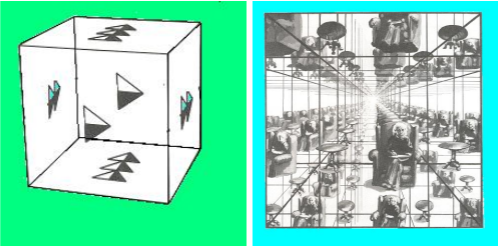
\includegraphics[scale=0.5]{images/geometria_universo/pagina_9_1.png}
\end{figure}

Es fácil ver que $\mathds{R}^3$ se puede rellenar con el cubo, y utilizando las identificaciones que nos da el 3-toro, que de por sí genera la geometría euclídea en dos dimensiones, tenemos que el 3-toro tendrá la geometría euclídea.

\item Describe otros dos universos tridimensionales obtenidos de un cubo por identificación de sus caras que tengan también geometría euclídea.

\underline{Otra identificación del cubo en 3 dimensiones:}

Sería un espacio parecido al anterior ya que su ``dominio fundamental'' está formada también por un cubo, pero esta vez con un cubo que tendría las siguientes identificaciones.

\begin{figure}[H]
\centering
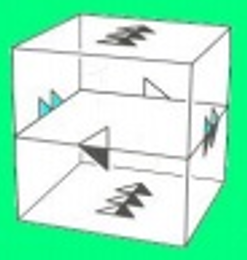
\includegraphics[scale=0.5]{images/geometria_universo/pagina_9_2.png}
\end{figure}

De esta forma vemos que podríamos decir que una de las caras está identificada de forma ``inversa''. En este caso si miramos hacia arriba o hacia uno de los lados sucedería lo mismo que en el toro, pero no es así en el caso de mirar hacia delante o hacia atrás. En este caso debemos de distinguir que al estar identificadas de esta manera si entramos por la parte de la derecha de una de las caras saldremos a la misma altura por la parte de la izquierda de la cara opuesta y viceversa en el caso de entrar por la parte de la izquierda de una de las caras. Entonces al rellenar todo R3 si nos situásemos en el centro del cubo nos veríamos a nosotros como en el Toro llano de 3 dimensiones, pero con la parte de la derecha en la izquierda y la de la izquierda en la derecha. 

\underline{Botella de Klein de 3 dimensiones:}

Volvemos a un espacio generado por un cubo en el cual identificamos las caras como se muestra en la siguiente imagen.

\begin{figure}[H]
\centering
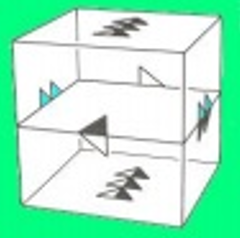
\includegraphics[scale=0.5]{images/geometria_universo/pagina_9_3.png}
\end{figure}

Con estas identificaciones volvemos al caso de antes, pero con una variación más, y es que cuando entramos por la cara delantera (o trasera) a parte de salir por la contraria invirtiendo izquierda y derecha también saldríamos baca abajo, es decir, lo que está arriba pasaría a estar abajo y lo que está abajo pasaría a estar arriba. La siguiente imagen puede ayudarnos a verlo más fácilmente.

\end{enumerate}

\vspace{0.5cm}

\textbf{Página 13}

\begin{enumerate}
\item Calcula para cada uno de los triángulos esféricos (en $\mathds{S}_R^2$) de la figura, la suma de sus ángulos y el área que encierran. Encuentra una fórmula que relacione la suma de los ángulos de un triángulo esférico y su área.


\begin{figure}[H]
	\centering
	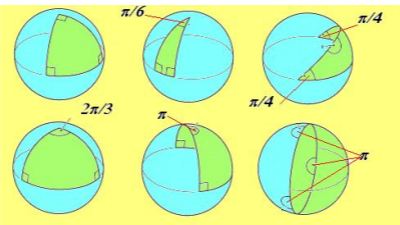
\includegraphics[scale=0.9]{images/geometria_universo/pagina_13_1.png}
\end{figure}

Empezamos calculando los de la primera fila y después los de la segunda. Representaremos la suma de los ángulos con $S$.

	\begin{enumerate}
	\item Cada ángulo es un \textit{ángulo recto} en la esfera, por tanto:
	\[S = \frac{\pi}{2}+\frac{\pi}{2}+\frac{\pi}{2}=\frac{3\pi}{2}\]
	En una esfera completa hay 8 triángulos como este, así que el área de uno de ellos es:
	\[A = \frac{4\pi R^2}{8} = \frac{\pi R^2}{2}\]
	
	\item Cada uno de los ángulos inferiores es un ángulo recto:
	\[S = \frac{\pi}{6}+\frac{\pi}{2}+\frac{\pi}{2}=\frac{7\pi}{6}\]
	Podemos poner $2\pi/\frac{\pi}{6}=12$ triángulos en una vuelta completa del hemisferio superior, y por tanto 24 en toda la esfera:
	\[A = \frac{4\pi R^2}{24} = \frac{\pi R^2}{6}\]
	
	\item Hay marcado un ángulo llano, que valdrá $\pi$.
	\[S = \frac{\pi}{4}+\frac{\pi}{4}+\pi=\frac{3\pi}{2}\]
	En la esfera completa hay $2\pi/\frac{\pi}{4}=8$ triángulos como este.
	\[A = \frac{4\pi R^2}{8} = \frac{\pi R^2}{2}\]
	
	\item Similar al \textit{b)}.
	\[S = \frac{2\pi}{3}+\frac{\pi}{2}+\frac{\pi}{2} = \frac{5\pi}{3}\]
	En un hemisferio hay $2\pi/\frac{2\pi}{3}=3$ triángulos como este, y en la esfera completa, 6.
	\[A = \frac{4\pi R^2}{6} = \frac{2\pi R^2}{3}\]
	
	\item De nuevo, ángulos rectos.
	\[S = \pi+\frac{\pi}{2}+\frac{\pi}{2}=2\pi\]
	Cuatro triángulos como este en la esfera.
	\[A = \frac{4\pi R^2}{4} = \pi R^2\]
		
	\item Tres ángulos que valen $\pi$:
	\[S=3\pi\]
	Dos hemisferios en la esfera:
	\[A=\frac{4\pi R^2}{2} = 2\pi R^2\]

	\end{enumerate}
	
Podemos ver que la relación de la suma de los ángulos con su área es:

\[A = (S-\pi)R^2 = E R^2,\]

donde $E$ es el exceso esférico.



\end{enumerate}

\vspace{0.5cm}

\textbf{Página 17}

\begin{enumerate}
\item Una sociedad de Planilandeses viven en una esfera de radio 1000 metros. La finca triangular de un granjero tiene por ángulos: $43'624^o$, $85'123^o$ y $51'270^o$ ¿Cuál es el área de la finca?


Como hemos visto anteriormente, el área del triángulo en la esfera viene dada por la siguiente fórmula $(\alpha + \beta + \gamma - \pi) \cdot R^2 = A(T)$ donde $\alpha$, $\beta$, $\gamma$ son los tres ángulos de dicho triangulo y $R$ el radio del mismo. Entonces para calcular este área primero pasamos los ángulos de grados a radianes:
\begin{align*}
\frac{43.624º \cdot (\pi \text{ rad} )}{180º} = 0.2424 \cdot \pi \text{ rad} \\
\frac{85.123º \cdot (\pi \text{ rad})}{180º} = 0.4729 \cdot \pi \text{ rad} \\
\frac{51.270º \cdot (\pi \text{ rad})}{180º} = 0.2848 \cdot \pi \text{ rad} \\
\end{align*}

Entonces aplicando la fórmula obtenemos que:

\[A(T) = (0.00009444 \cdot \pi) \cdot 10002 = 296.70597  \text{ m}^2\]

\item Un triángulo esférico de área $5410.52 \text{m}^2$
tiene por ángulos $60.0013º$, $60.007º$ y $60.0011º$. ¿Cuál es el radio de la esfera?

Primero pasamos los ángulos a radianes y después utilizando la misma fórmula del ejercicio anterior despejamos el radio:
\begin{align*}
\frac{60.0013º \cdot (\pi \text{ rad})}{180º} = 0.3333 \cdot \pi \text{ rad} \\
\frac{60.007º \cdot (\pi \text{ rad})}{180º} = 0.3334 \cdot \pi \text{ rad} \\
\frac{60.0011º (\pi \text{ rad})}{180º} = 0.3333 \cdot \pi \text{ rad} \\
R = (\frac{5410.52}{0.0001641})^{1/2} = 5742.710097 \text{ m}
\end{align*}


\item ¿Cuánto suman los ángulos de un polígono esférico de $n$ lados?

Para responder a esta pregunta vamos a utilizar un teorema, el cual vimos anteriormente en teoría, que viene a decir lo siguiente: 

\begin{center}
\textit{Toda triangulación de un polígono con $n$ vértices\\tiene $n-2$ triángulos y $n-3$ diagonales.}
\end{center}

Por lo tanto, nuestro polígono esférico de $n$ lados tendrá $n$ vértices y por tanto $n-2$ triángulos esféricos. Es fácil ver que la suma de los ángulos internos de nuestro polígono esférico coincide con la suma de los ángulos de los triángulos esféricos que hemos obtenido al triangular nuestro polígono. En consecuencia, como sabemos que la suma de los ángulos de todo triángulo esférico es $\geq180º$ llegamos a la conclusión que la suma de los ángulos de un polígono esférico de $n$ lados será $\geq$ $(n-2) \cdot 180º$.

\end{enumerate}

\vspace{0.5cm}

\textbf{Página 20}

\begin{enumerate}
\item Explica la siguiente visualización de $\mathds{P}^3$. ¿Es $\mathds{P}^3$ orientable?

\begin{figure}[H]
	\centering
	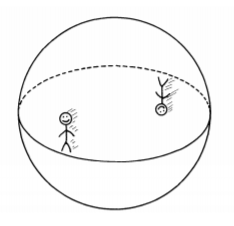
\includegraphics[scale=0.8]{images/geometria_universo/pagina_20_1.png}
\end{figure}

Podemos considerar 2 hemisferios, el superior y el inferior, por ello, cuando la persona sale por el hemisferio inferior, entra por el superior ya que los puntos antípodas del borde están identificados de forma opuesta.

Sabemos por un teorema que $\mathds{P}^n$ es orientable $\Longleftrightarrow$ $n$ es impar, por tanto $\mathds{P}^3$ es orientable.

\end{enumerate}


\vspace{0.5cm}

\textbf{Página 33}

\begin{enumerate}
\item En un plano hiperbólico de curvatura $-1$, ¿cuál es el área de
un triángulo de ángulos $\pi/3$,  $\pi/4$ y  $\pi/6$?

Sabemos que:

\[
\rho = \frac{1}{\sqrt{-k}} = 1
\] 

Por otro lado:

\[
A(t)=\rho^2(\pi -(\alpha+\beta+\gamma)) = (\pi -(\alpha+\beta+\gamma)) = \pi - \frac{3\pi}{4} =\frac{\pi}{4}
\]

\item  ¿Cuánto suman los ángulos de un polígono hiperbólico de $n$ lados?

Sabemos que la suma de los ángulos de un triángulo hiperbólico es menor que $\pi$, y por tanto, procediendo del mismo modo que para la geometría euclídea, para cualquier $n$ tendremos que la suma de un polígono hiperbólico de $n$ lados será menor que $(n-2)\cdot\pi$.


\end{enumerate}

\vspace{0.5cm}


\textbf{Página 42}

\begin{enumerate}
\item Para cada uno de los universos descritos en la figura, determina cómo se unen las esquinas. ¿Cuáles tienen geometría elíptica, hiperbólica o euclídea?

\begin{figure}[H]
	\centering
	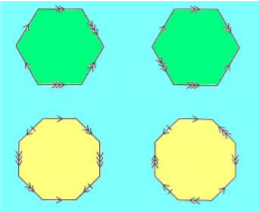
\includegraphics[scale=1]{images/geometria_universo/pagina_42_1.png}
\end{figure}

Veamos como se unen las esquinas en los hexágonos superiores:

\begin{figure}[H]
\centering
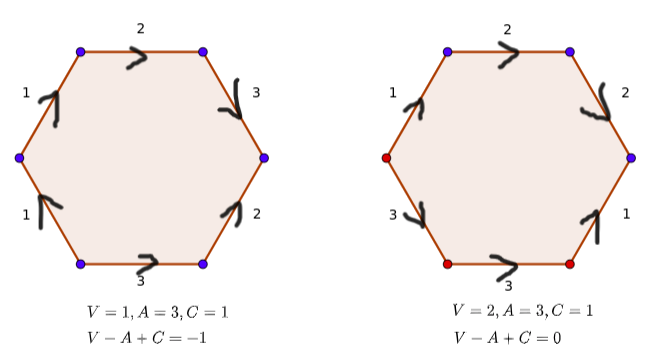
\includegraphics[scale=0.4]{images/geometria_universo/pagina_42_ej_1_a.png}
\end{figure}

Primero de todo, recordemos que el ángulo de un vértice en un hexágono es $\frac{2\pi}{3}$.

En el primer caso, tenemos que todos los vértices van al mismo punto ($6\frac{2\pi}{3}>2\pi$), por lo que tendremos un único vértice formando lo opuesto a un de un punto cónico, y la geometría será la hiperbólica.

En el segundo caso, los vértices se juntan de tres en tres ($3\frac{2\pi}{3}=2\pi$), estando en el caso de geometría euclídea.

\begin{figure}[H]
\centering
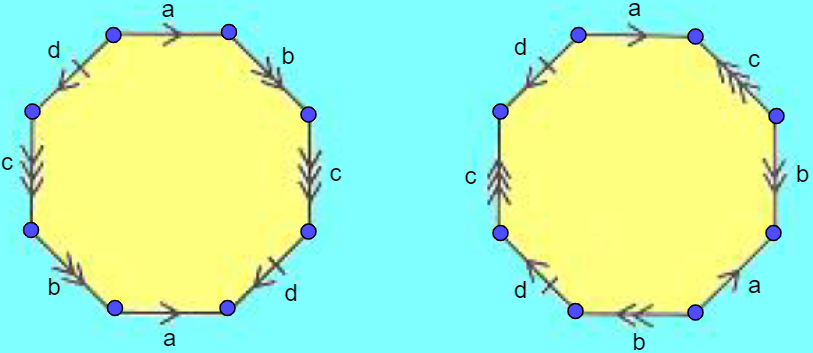
\includegraphics[scale=0.55]{images/geometria_universo/pagina_42_ej_1_b.png}
\end{figure}

Para los dos octógonos, cuyo ángulo en cada vértice es $\frac{3\pi}{4}$, tenemos que todos los vértices van al mismo punto y forman lo opuesto a un punto cónico ($8\frac{3\pi}{4}>2\pi$) por tanto en los dos casos nos encontramos con la topología hiperbólica.


\item Determina cuál es la geometría de un universo que sea suma conexa de $m$ toros con $m\geq2$.

Imaginémonos la figura de la imagen, pero reflejada respecto de los dos planos (forma como un hueso, con agujeros en las 4 puntas).

\begin{figure}[H]
\centering
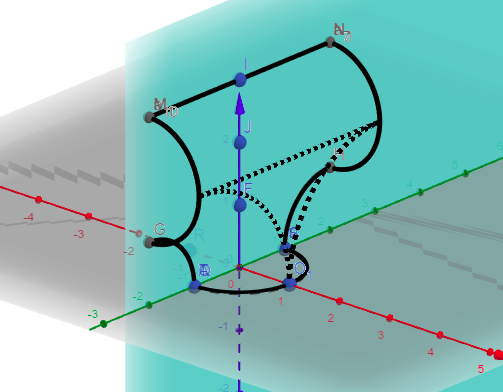
\includegraphics[scale=0.55]{images/geometria_universo/pagina_42_ej_2.png}
\end{figure}

Si esta figura la insertamos en el agujero del centro de la figura que vemos a continuación, tendríamos un 4-toro.

\begin{figure}[H]
\centering
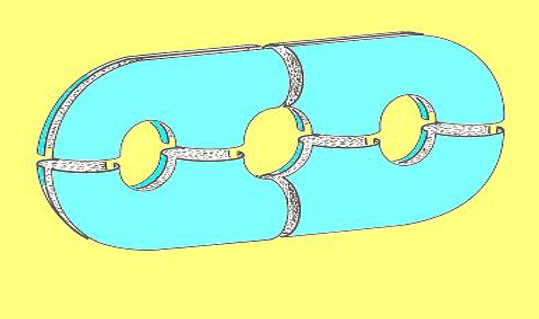
\includegraphics[scale=0.35]{images/geometria_universo/fig_pag_41.png}
\end{figure}


Como ya hemos visto que el 3-toro tiene geometría hiperbólica, solo queda ver qué pasa con esa figura que añadimos.

Podemos ver que cada una de las 4 partes que hemos añadido tiene 6 lados, lo cual deformándolos adecuadamente llegamos a unos hexágonos del mismo tipo que los mencionados en la página 41 de los apuntes de la asignatura, luego en consecuencia obtenemos que el 4-toro tiene geometría hiperbólica.

Si esto proceso lo volvemos a aplicar con el 4-toro, obtenemos del mismo modo un 5-toro con geometría hiperbólica. Aplicamos esto indefinidamente y obtenemos que todos los n-toros tienen geometría hiperbólica.

\end{enumerate}




\newpage
\begin{thebibliography}{X}

\bibitem{1} \textsc{Apuntes de Clase}

\end{thebibliography}


\end{document}

